\section{Linear Stability Analysis of Interfaces in Porous Media}
\label{sec:lsa}

This chapter develops the asymptotic analysis and linear stability modeling for the interface between two immiscible fluids in a porous medium (or equivalently, in a Hele--Shaw cell). The formulation is structured in two parts. The first encompasses classical hydrodynamic instabilities driven by viscous gradients and capillary forces (Saffman--Taylor instability), and the second addresses the instability interaction when an external magnetic field is applied to a ferrofluid.

\medskip
\noindent\textbf{Notation.} Throughout this chapter the symbol $\Phi$ denotes the (hydrodynamic) velocity potential, with the convention $\mathbf{v} = \nabla\Phi$. This is distinct from the Cahn--Hilliard order parameter $\phi$ employed in Chapters on the theoretical background and on the LBM computational methodology, which represents a phase-field indicator and is unrelated to the velocity potential introduced here.

\subsection{Physical Description of the System and Nomenclature}

The macroscopic system consists of two viscous and incompressible fluids confined in a homogeneous and isotropic porous medium. A Cartesian coordinate system is defined wherein the $y$-direction is orthogonal to the planar wave interface.

\textbf{Fluid 1} (the invading fluid) is located in the lower region ($y < 0$) and is injected with a uniform filtration velocity $V/\epsilon$ in the positive vertical direction ($\hat{\jmath}$). In the first case, it behaves as a standard Newtonian fluid, whereas in the second case, it is a ferrofluid; in both scenarios, it displaces \textbf{Fluid 2} (the defending fluid), which is Newtonian and situated in the upper region ($y > 0$). The system is subject to gravitational acceleration acting in the $-y$ direction. This physical configuration is depicted in the figure below.

\begin{figure}[htbp]
  \centering
  \framebox{\parbox{0.8\textwidth}{\centering
    \vspace{3cm}
    \textbf{Image Placeholder} \\
    \small\textit{Schematic representation of the flow and the perturbed interface.}
    \vspace{3cm}
  }}
  \caption{Schematic representation of the flow and the perturbed interface between the invading (lower) and defending (upper) fluids in the porous medium.}
  \label{fig:physical_scheme}
\end{figure}

The interface position, in both cases, is defined by Equation~\ref{eq:interface_pos}:
\begin{equation} \label{eq:interface_pos}
    y(x,t) = \frac{V}{\epsilon} t + \lambda(x,t),
\end{equation}
where $y$ denotes the vertical position, $(V/\epsilon)\,t$ is the mean position of the interface moving with constant velocity, and $\lambda(x,t)$ represents the perturbation (distortion) at the interface.

The formulation relies on the macroscopic sharp-interface approximation. This theoretical idealization is valid under the assumption of high Péclet numbers ($Pe \gg 1$), where convective transport dominates molecular diffusion, thereby suppressing dynamic mixing between the immiscible phases and confining interfacial gradients to a negligibly thin region.

\subsection{Development of the Kinematic Equation}

The temporal evolution of the boundary between the fluids is governed by the kinematic boundary condition. Physically, this formulation establishes that the interface acts as a continuous material surface; that is, there is no mass flux (or fluid crossover) through it. This ensures that any fluid particle originally located at the interface remains constrained to this geometric boundary throughout the flow. To mathematically model this restriction, the position of the moving boundary is implicitly described by a scalar function $F(x,y,t) = 0$. Considering the system in a stationary reference frame, where the base state of the (planar) interface is displaced with a constant mean velocity $V/\epsilon$ in the vertical $y$-direction, and upon which a perturbation denoted by $\lambda (x,t)$ is superimposed, the surface topology is rigorously defined by Equation~\ref{eq:interface_evolution}:

\begin{equation}
\label{eq:interface_evolution}
F(x,y,t) = y - \left( \frac{V t}{\epsilon} + \lambda(x,t) \right) = 0.
\end{equation}

The strict requirement that a fluid element does not leave the interface implies, under the Lagrangian formulation, that the rate of change of $F$ following the fluid particle's motion must be identically zero. Consequently, the material (or convective) derivative of the surface function vanishes at the boundary, ensuring that the geometric propagation velocity of the interface is perfectly coupled with the local velocity of the flow field $\mathbf{v}$. This fundamental condition is expressed by Equation~\ref{eq:material_derivative_F}:

\begin{equation}
\label{eq:material_derivative_F}
    \frac{D F}{D t} = \frac{\partial F}{\partial t} + \mathbf{v} \cdot \nabla F = 0.
\end{equation}

Restricting the formulation to a two-dimensional flow with velocity field $\mathbf{v} = (v_x, v_y)$, the expansion of the material derivative operator requires the explicit evaluation of the temporal and spatial partial derivatives of $F(x,y,t)$. Following these procedures, the vertical component of the fluid velocity ($v_y$) at the boundary can be evaluated by Equation~\ref{eq:vertical_velocity_boundary}:

\begin{equation}
\label{eq:vertical_velocity_boundary}
    v_y = \frac{\partial \lambda}{\partial t} + v_x \frac{\partial \lambda}{\partial x} + \frac{V}{\epsilon}.
\end{equation}

According to Darcy's Law, the velocity vector is directly proportional to the pressure gradient ($\mathbf{v} \propto \nabla p$). As the curl operator applied to any gradient field is identically zero ($\nabla \times \nabla p = \mathbf{0}$), irrotationality is intrinsic to the system, ensuring the existence of a scalar potential $\Phi$ that describes the velocity field ($\mathbf{v} = \nabla \Phi$). Applying this to Equation~\ref{eq:vertical_velocity_boundary} consolidates a kinematic boundary partial differential equation, valid for the interface between the fluids, as described by Equation~\ref{eq:PDE_Interface}:

\begin{equation}
\label{eq:PDE_Interface}
    \frac{\partial \lambda}{\partial t} + \frac{\partial \Phi}{\partial x} \frac{\partial \lambda}{\partial x} + \frac{V}{\epsilon} = \frac{\partial \Phi}{\partial y}.
\end{equation}

\subsection{Equilibrium Solution}

The equilibrium (base) state of the system corresponds to the unperturbed configuration $\lambda(x,t) \equiv 0$, in which the interface remains strictly planar and translates uniformly with the prescribed filtration velocity $V/\epsilon$ in the $+\hat{\jmath}$ direction. The full velocity potential and pressure field associated with this base state must be derived explicitly before the perturbation analysis can be linearized around it.

\subsubsection{Base Velocity Potential}

In the equilibrium configuration, the velocity field in each phase reduces to the uniform plug flow
\begin{equation}
\label{eq:base_velocity}
\mathbf{v}_j^0 = \frac{V}{\epsilon}\,\hat{\jmath},\qquad j = 1, 2.
\end{equation}
Since the flow in porous media is irrotational under Darcy's law, this base velocity is the gradient of a scalar potential, $\mathbf{v}_j^0 = \nabla \Phi_j^0$. Direct integration of the constant vertical component of $\mathbf{v}_j^0$ yields the linear base potential:
\begin{equation}
\label{eq:base_potential}
\Phi_j^0(y, t) = \frac{V}{\epsilon}\,y + g_j(t),
\end{equation}
where $g_j(t)$ is an arbitrary function of time fixed by the choice of gauge. Since only the gradient of $\Phi_j^0$ enters the physical equations, $g_j(t)$ does not affect the subsequent analysis.

\subsubsection{Base Pressure Profile}

Substituting the base velocity field~\eqref{eq:base_velocity} into the extended Darcy's law for each phase yields a one-dimensional ordinary differential equation for the base pressure $p_j^0(y)$,
\begin{equation}
\label{eq:base_pressure_ode}
\frac{\partial p_j^0}{\partial y} = -\frac{\mu_j}{k_j}\,\frac{V}{\epsilon} \;-\; \rho_j\, g.
\end{equation}
Direct integration along the vertical coordinate gives the base pressure profile in each phase:
\begin{equation}
\label{eq:base_pressure}
p_j^0(y) = p_{\mathrm{ref},j} \;-\; \rho_j\, g\, y \;-\; \frac{\mu_j}{k_j}\,\frac{V}{\epsilon}\, y,
\end{equation}
where $p_{\mathrm{ref},j}$ is a reference pressure constant fixed by the upstream and downstream boundary conditions of each domain. The base state therefore contains two distinct contributions to the longitudinal pressure variation: a hydrostatic gradient $-\rho_j g$ and a viscous (Darcy) gradient $-(\mu_j/k_j)(V/\epsilon)$ associated with the uniform filtration.

\subsubsection{Consistency with the Boundary Conditions}

Two checks are required to confirm that the base state defined by~\eqref{eq:base_potential}--\eqref{eq:base_pressure} is internally consistent with both the kinematic and the dynamic boundary conditions evaluated at the unperturbed interface position $y_{\mathrm{int}}(t) = (V/\epsilon)\,t$.

\paragraph{Kinematic condition.} The general kinematic relation~\eqref{eq:PDE_Interface} evaluated at $\lambda \equiv 0$ reduces to
\begin{equation}
\frac{V}{\epsilon} \;=\; \frac{\partial \Phi_j^0}{\partial y} \;=\; \frac{V}{\epsilon},
\end{equation}
which is satisfied identically for both phases. The base state therefore corresponds to a self-consistent rigid translation of the planar interface.

\paragraph{Dynamic condition.} Subtracting the two base pressure profiles~\eqref{eq:base_pressure} evaluated at the moving interface $y_{\mathrm{int}}(t)$ gives
\begin{equation}
\label{eq:base_pressure_jump}
p_2^0 - p_1^0 \,\Big|_{y_{\mathrm{int}}}
\;=\; (p_{\mathrm{ref},2} - p_{\mathrm{ref},1})
\;+\; \left[\,(\rho_1 - \rho_2)\,g \;+\; \frac{V}{\epsilon}\!\left(\frac{\mu_1}{k_1} - \frac{\mu_2}{k_2}\right)\right]\,\frac{V}{\epsilon}\,t.
\end{equation}
Since the unperturbed planar interface has zero curvature ($c \equiv 0$), the dynamic boundary condition requires the pressure jump $p_2^0 - p_1^0$ to vanish on the interface. This is enforced by gauge-fixing the reference pressures such that
\begin{equation}
\label{eq:gauge_fixing}
p_{\mathrm{ref},2} - p_{\mathrm{ref},1}
\;=\; -\!\left[\,(\rho_1 - \rho_2)\,g \;+\; \frac{V}{\epsilon}\!\left(\frac{\mu_1}{k_1} - \frac{\mu_2}{k_2}\right)\right]\,\frac{V}{\epsilon}\,t.
\end{equation}
The time-dependent base-state offset is therefore absorbed into the choice of reference pressures and does not enter the perturbation analysis. The perturbation framework that follows considers only the linearized deviations $\Phi'$, $p'$, and $\lambda$ from this self-consistent base state.

\subsection{Linearization of the Kinematic Equation}

\subsubsection{Velocity Potential Perturbation}

To investigate the evolution of instabilities at the boundary, a linear perturbation analysis is applied. The total velocity potential field is decomposed into the superposition of the base state $\Phi^0$, derived in the previous subsection, and an infinitesimal spatiotemporal fluctuation $\Phi'$, as shown in Equation~\ref{eq:potential_decomp}:

\begin{equation} \label{eq:potential_decomp}
    \Phi(x,y,t) = \Phi^0(y,t) + \Phi'(x,y,t).
\end{equation}

The incompressibility of the fluids ($\nabla \cdot \mathbf{v} = 0$) requires the perturbation potential to satisfy Laplace's equation in both domains. Physically, since the hydrodynamic fluctuations are induced strictly by the local instability of the interface, the mathematical condition of asymptotic decay at infinity is imposed. With Fluid 1 in the lower domain and Fluid 2 in the upper domain, this is formulated as Equations~\ref{eq:laplace} and~\ref{eq:bcs_infinity}:

\begin{equation} \label{eq:laplace}
    \nabla^2 \Phi_1' = 0 \quad \text{and} \quad \nabla^2 \Phi_2' = 0,
\end{equation}
\begin{equation} \label{eq:bcs_infinity}
    \Phi_1' \to 0 \text{ as } y \to -\infty, \qquad \Phi_2' \to 0 \text{ as } y \to +\infty.
\end{equation}

\subsubsection{Linearization of the Kinematic Condition}

The linearization proceeds by inserting the decomposed potential into the general kinematic equation~\eqref{eq:PDE_Interface}. Under the assumption of infinitesimal perturbations, products between fluctuating terms (e.g., $\frac{\partial \Phi'}{\partial x}\frac{\partial \lambda}{\partial x}$) constitute higher-order quantities and are thus neglected. Evaluating this expression at the base-state interface position ($y \approx Vt/\epsilon$), the terms governing the constant translation of the reference frame cancel out by virtue of the base state derived in the previous subsection. Consequently, the resulting linearized kinematic condition directly correlates the temporal growth rate of the perturbation with the vertical component of the perturbed velocity field, presented in Equation~\ref{eq:kinematic_linear}:

\begin{equation} \label{eq:kinematic_linear}
    \frac{\partial \lambda}{\partial t} = \frac{\partial \Phi'}{\partial y}.
\end{equation}

The linear stability analysis of the interface proceeds through the decomposition of perturbations into normal modes. The wavenumber $\alpha$, which characterizes the spatial periodicity, and the complex growth rate $s$ are introduced in Equation~\ref{eq:normal_modes}:

\begin{equation} \label{eq:normal_modes}
    \alpha = \frac{2\pi}{\lambda_w}, \qquad s = \zeta - i\omega,
\end{equation}
where $\lambda_w$ is the perturbation wavelength, $\zeta$ quantifies the exponential amplification factor (stability criterion), and $\omega$ represents the temporal oscillatory component. An ansatz is postulated for the fluctuations in the form of two-dimensional harmonic waves, formulated in Equation~\ref{eq:ansatz}:

\begin{equation} \label{eq:ansatz}
\begin{aligned}
\lambda(x,t) &= \lambda_0 \,e^{i\alpha x + st}, \\
\Phi_1'(x,y,t) &= A_1(y) \,e^{i\alpha x + st} \qquad (y < y_0), \\
\Phi_2'(x,y,t) &= A_2(y) \,e^{i\alpha x + st} \qquad (y > y_0).
\end{aligned}
\end{equation}

Inserting these modal solutions into Laplace's equation ($\nabla^2 \Phi' = 0$) converts the partial differential equation into a second-order ordinary differential equation for the vertical amplitude, given by Equation~\ref{eq:ode}:

\begin{equation} \label{eq:ode}
    \frac{d^2 A_j}{dy^2} - \alpha^2 A_j = 0.
\end{equation}

By imposing the physical requirement of asymptotic decay of the perturbations at the far-field limit from the boundary ($\Phi' \to 0$ as $y \to \pm \infty$), only the bounded solutions are selected in Equation~\ref{eq:bounded_sols}:

\begin{equation} \label{eq:bounded_sols}
    A_1(y) = C_1 \,e^{+\alpha(y - y_0)}, \qquad A_2(y) = C_2 \,e^{-\alpha(y - y_0)}.
\end{equation}

\subsubsection{Application of the Kinematic Condition}

Closure of the system requires determining the integration constants $C_1$ and $C_2$ via the linearized kinematic condition $\frac{\partial \lambda}{\partial t} = \frac{\partial \Phi'}{\partial y}$ evaluated at the unperturbed interface $y = y_0$. Under the normal mode representation, differential operations translate into the algebraic mapping $\partial_t \to s$ and $\partial_y \to \pm \alpha$. Applying these relations to the boundary condition yields the integration constants as functions of the growth rate and wavenumber. Consequently, the perturbed potential fields become uniquely coupled to the amplitude of the geometric deformation $\lambda_0$, yielding Equation~\ref{eq:phi_sols}:

\begin{equation} \label{eq:phi_sols}
\begin{aligned}
\Phi_1' &= \;+\,\frac{s}{\alpha}\,\lambda_0 \,e^{+\alpha(y-y_0)} \,e^{i\alpha x + st}, \\
\Phi_2' &= \;-\,\frac{s}{\alpha}\,\lambda_0 \,e^{-\alpha(y-y_0)} \,e^{i\alpha x + st}.
\end{aligned}
\end{equation}

\subsection{Dynamic Boundary Condition for the Non-Magnetic Case}

The pressure in each fluid is governed by the extended Darcy's law (accounting for gravitational potential). The relationship between pressure and velocity potential for fluids 1 and 2 is defined in Equations~\ref{eq:extended_darcy_1} and~\ref{eq:extended_darcy_2}:

\begin{align}
    p_1 &= -\frac{\mu_1}{k_1} \Phi_1 + \rho_1 \mathbf{g} \cdot \mathbf{x}, \label{eq:extended_darcy_1} \\
    p_2 &= -\frac{\mu_2}{k_2} \Phi_2 + \rho_2 \mathbf{g} \cdot \mathbf{x}. \label{eq:extended_darcy_2}
\end{align}

The dynamic boundary condition requires the pressure jump across the interface to be balanced by surface tension, as stated in Equation~\ref{eq:pressure_jump}:
\begin{equation} \label{eq:pressure_jump}
    p_2 - p_1 = \sigma c,
\end{equation}
where the linearized curvature is $c \approx \frac{\partial^2 \lambda}{\partial x^2}$.

\subsubsection{Linearization via Taylor Expansion of the Base Pressure}

The substitution of the pressure expressions into the dynamic boundary condition must be performed at the perturbed interface position $y = (V/\epsilon)\,t + \lambda$, not at the unperturbed position $(V/\epsilon)\,t$. A Taylor expansion of the base pressure profile~\eqref{eq:base_pressure} around the unperturbed interface, retained to first order in $\lambda$, yields
\begin{equation}
\label{eq:taylor_base}
p_j^0\!\left(\tfrac{V}{\epsilon}t + \lambda\right)
\;\approx\; p_j^0\!\left(\tfrac{V}{\epsilon}t\right) \;+\; \lambda\,\frac{\partial p_j^0}{\partial y}\bigg|_{y_{\mathrm{int}}}
\;=\; p_j^0\!\left(\tfrac{V}{\epsilon}t\right) \;-\; \lambda\!\left(\rho_j\, g \;+\; \frac{\mu_j}{k_j}\,\frac{V}{\epsilon}\right),
\end{equation}
where the second equality follows from the base-state ODE~\eqref{eq:base_pressure_ode}. The total perturbed pressure at the interface is therefore
\begin{equation}
\label{eq:perturbed_total_p}
p_j\!\left(\tfrac{V}{\epsilon}t + \lambda\right)
\;=\; p_j^0\!\left(\tfrac{V}{\epsilon}t\right)
\;-\; \lambda\!\left(\rho_j\, g \;+\; \frac{\mu_j}{k_j}\,\frac{V}{\epsilon}\right)
\;-\; \frac{\mu_j}{k_j}\,\Phi_j',
\end{equation}
where the third term on the right-hand side is the perturbation of the pressure coming from the perturbed velocity potential $\Phi_j'$ through Darcy's law.

Substituting~\eqref{eq:perturbed_total_p} into the pressure-jump condition~\eqref{eq:pressure_jump}, applying the gauge-fixing~\eqref{eq:gauge_fixing} that absorbs the zeroth-order base-state offset, and collecting the first-order terms, yields the linearized dynamic boundary condition:
\begin{equation} \label{eq:dynamic_linear}
    \frac{\mu_1}{k_1}\, \Phi_1' \;-\; \frac{\mu_2}{k_2}\, \Phi_2'
    \;+\; \left[\, \frac{V}{\epsilon}\!\left(\frac{\mu_1}{k_1} - \frac{\mu_2}{k_2}\right)
    \;-\; g(\rho_2 - \rho_1)\,\right]\,\lambda
    \;=\; \sigma\, \frac{\partial^2 \lambda}{\partial x^2}.
\end{equation}
The bracketed term collects the destabilizing contributions of the viscous (Darcy) mismatch and of gravity, while the right-hand side represents the stabilizing capillary force.

\subsubsection{Dispersion Relation}

Inserting the modal solutions~\eqref{eq:phi_sols} for $\Phi_1', \Phi_2'$, and the corresponding mode $\lambda = \lambda_0\,e^{i\alpha x + st}$ into the linearized dynamic condition~\eqref{eq:dynamic_linear}, and factoring out the common harmonic dependence, reduces the differential equation to an algebraic dispersion relation. Solving for the complex growth rate $s = \zeta - i\omega$ yields Equation~\ref{eq:dispersion_dimensional}:

\begin{equation} \label{eq:dispersion_dimensional}
    \zeta - i\omega = \frac{\alpha}{\dfrac{\mu_1}{k_1} + \dfrac{\mu_2}{k_2}}
    \left[\, \frac{V}{\epsilon}\!\left( \frac{\mu_2}{k_2} - \frac{\mu_1}{k_1} \right)
    \;+\; g(\rho_2 - \rho_1) \;-\; \sigma \alpha^2 \,\right].
\end{equation}

\subsubsection{Analysis of the Real and Imaginary Parts}

Since all terms on the right-hand side of Eq.~\ref{eq:dispersion_dimensional} are purely real (viscosity, permeability, density, and surface tension), it follows:

\begin{itemize}
    \item \textbf{Imaginary Part ($\omega$):} As shown in Equation~\ref{eq:imaginary_part}:
    \begin{equation} \label{eq:imaginary_part}
        \omega = 0.
    \end{equation}
    This indicates that the principle of exchange of stabilities holds: the perturbation is non-oscillatory and grows or decays monotonically. This strictly monotonic evolution reflects the highly dissipative nature of flow in porous media. In the Darcy regime (creeping flow, $\mathrm{Re} \ll 1$), inertial forces are entirely negligible compared to viscous drag from the porous matrix. Consequently, the system lacks the kinetic-energy storage mechanism required to sustain inertial oscillations or traveling waves, behaving analogously to a strongly overdamped oscillator.

    \item \textbf{Real Part ($\zeta$):} Expressed in Equation~\ref{eq:real_part}:
    \begin{equation} \label{eq:real_part}
        \zeta = \frac{\alpha}{\dfrac{\mu_1}{k_1} + \dfrac{\mu_2}{k_2}}
        \left[\, \underbrace{\frac{V}{\epsilon}\!\left( \frac{\mu_2}{k_2} - \frac{\mu_1}{k_1} \right)}_{\text{viscous forcing}}
        \;+\; \underbrace{g(\rho_2 - \rho_1)}_{\text{gravity}}
        \;-\; \underbrace{\sigma \alpha^2}_{\text{capillarity}} \,\right].
    \end{equation}
\end{itemize}

\subsubsection{Nondimensionalization}

To construct a generalized parametric space, the system is nondimensionalized. The characteristic velocity scale is defined by the uniform filtration velocity $U \equiv V/\epsilon$. The characteristic length scale $b$ is selected based on the specific geometry, representing either the macroscopic characteristic length of the porous domain or the gap thickness in the Hele--Shaw cell analog. This physical selection establishes the convective timescale $T = b/U$.

Defining the characteristic length scale $b$, velocity $U$, and time $T = b/U$, the dimensionless variables are defined in Equation~\ref{eq:nondim_vars}:
\begin{equation} \label{eq:nondim_vars}
    \zeta^* = \zeta\,\frac{b}{U}, \qquad \alpha^* = \alpha\, b.
\end{equation}

Assuming a homogeneous medium ($k_1 = k_2 = k$) and defining the viscosity ratio $M = \mu_2/\mu_1$, the equation can be rewritten using the following dimensionless numbers:
\begin{itemize}
    \item $\mathrm{Ca} = \dfrac{\mu U}{\sigma}$ (capillary number),
    \item $\mathrm{Bo} = \dfrac{\Delta \rho\, g\, b^2}{\sigma}$ (Bond number),
    \item $\mathrm{Da} = \dfrac{k}{b^2}$ (Darcy number).
\end{itemize}

The final dimensionless dispersion relation becomes Equation~\ref{eq:dispersion_nondim}:
\begin{equation} \label{eq:dispersion_nondim}
    \zeta^*(\alpha^*) = \alpha^*\,\frac{M-1}{M+1}
    \;+\; \frac{\mathrm{Da}}{\mathrm{Ca}\,(1+M)}\,\alpha^*\,(\mathrm{Bo} - {\alpha^*}^2).
\end{equation}

\subsubsection{Graphical Analysis of the Equation}

Figure~\ref{fig:Simple-LSA-graphic} shows the dispersion relation plot obtained from the linear stability analysis governing the system described in Equation~\ref{eq:dispersion_nondim}. The dynamic stability of the interface is determined by the sign of the dimensionless growth rate, $\zeta^*$. Configurations with $\zeta^* > 0$ indicate amplification of interfacial perturbations in time, which characterizes the unstable regime. In contrast, the semi-plane $\zeta^* < 0$ defines the asymptotically stable region, where fluctuations are strictly damped. It is also observed that, for large dimensionless wavenumbers ($\alpha^* \gg 1$), the curve shows a sharp parabolic decay toward negative infinity ($\zeta^* \to -\infty$). Analytically, this behavior is governed by the dominance of the negative third-order polynomial term ($-{\alpha^*}^3$) in the dispersion relation (Equation~\ref{eq:dispersion_nondim}). Physically, this decay reflects the restraining effect of surface tension: at microscopic length scales (high $\alpha^*$), the increase in interfacial curvature generates extreme capillary pressure gradients that act as a dominant restoring force, rapidly suppressing the growth of short waves and ensuring the stabilization of the system in this limit.

\begin{figure}
    \centering
    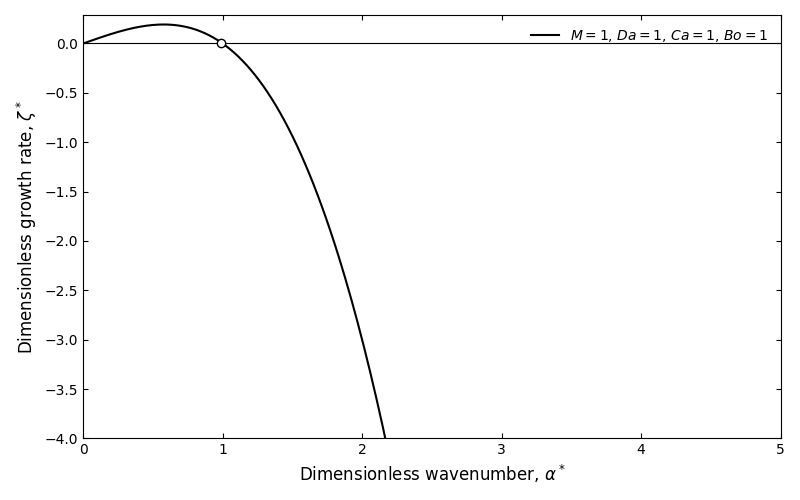
\includegraphics[width=0.5\linewidth]{figuras/lsa/Grafico-LSA-uma-linha-DaCaBoM-1.png}
    \caption{Dimensionless dispersion relation $\zeta^*(\alpha^*)$ for the non-magnetic Saffman--Taylor configuration. Positive values indicate growth of the perturbation (unstable regime); negative values indicate damping (stable regime).}
    \label{fig:Simple-LSA-graphic}
\end{figure}

Figure~\ref{fig:Simple-LSA-graphic-per-term} illustrates the individual contributions of the physical mechanisms governing the interfacial stability. The total dimensionless growth rate ($\zeta^*$) is the linear superposition of viscous, gravitational, and capillary effects.

As shown in the plot, the viscous forcing and gravity terms exhibit a linear dependence on the dimensionless wavenumber ($\alpha^*$). Under the evaluated unstable conditions ($M > 1$ and $\mathrm{Bo} > 0$), both act as purely destabilizing forces. If acting alone, they would promote continuous and unbounded growth of perturbations across all spatial scales.

Conversely, the capillarity term provides the essential stabilizing mechanism. It scales with the negative cube of the wavenumber ($-{\alpha^*}^3$). The graph clearly demonstrates the physical interplay between these forces across the spectrum:

\begin{itemize}
    \item \textbf{Long-wave regime (low $\alpha^*$):} the linear destabilizing forces (viscosity and gravity) dominate, causing the total growth rate to increase and driving the macroscopic instability of the interface.
    \item \textbf{Short-wave regime (high $\alpha^*$):} as the wavenumber increases, the wavelength decreases, resulting in a highly curved interface. In this region, the cubic capillary term rapidly outpaces the linear components.
\end{itemize}
This dynamic explains the characteristic parabolic shape of the total growth rate curve. The system reaches a peak of maximum instability before undergoing a sharp decline. Exactly where the capillary damping equals the combined viscous and gravitational forces, the total curve crosses the horizontal axis ($\zeta^* = 0$). Beyond this cut-off wavenumber, the surface tension acts as a strict low-pass filter, completely suppressing microscopic perturbations.

\begin{figure}
    \centering
    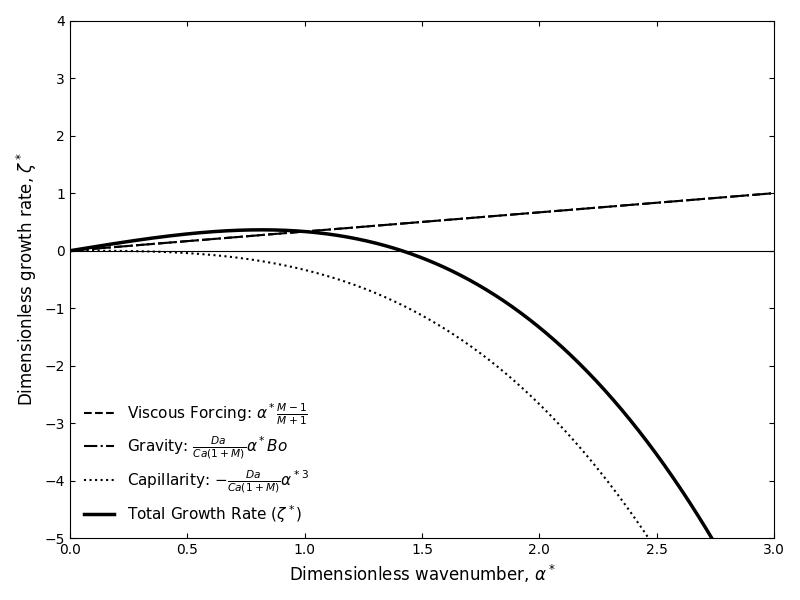
\includegraphics[width=0.5\linewidth]{figuras/lsa/Grafico-LSA-Impacto-de-cada-termo.png}
    \caption{Individual contributions of the viscous, gravitational, and capillary terms to the dimensionless growth rate $\zeta^*(\alpha^*)$ in the non-magnetic Saffman--Taylor case.}
    \label{fig:Simple-LSA-graphic-per-term}
\end{figure}

\subsection{Dynamic Boundary Condition for the Magnetic Case}

The introduction of an external magnetic field modifies the stress balance at the interface due to the polarization of the ferrofluid (Fluid 1). To prevent notational ambiguity with the dynamic viscosity ($\mu$), the absolute magnetic permeability of the fluids is denoted herein by $\mu_{m1}$ and $\mu_{m2}$. Since Fluid 2 is an ordinary, non-magnetic Newtonian fluid, its permeability equals that of the vacuum ($\mu_{m2} = \mu_0$).

\subsubsection{Extended Darcy's Law and Pressure Jump}

The momentum equation for the ferrofluid is governed by the extended Darcy's law, which incorporates both the gravitational potential and the Kelvin body force arising from the gradient of the magnetic energy:
\begin{equation} \label{eq:darcy_magnetic}
    \frac{\mu_1}{k}\, \mathbf{v}_1 = -\nabla p_1 + \rho_1 \mathbf{g} + \mu_0 \chi_1 \nabla \!\left( \tfrac{1}{2} H^2 \right).
\end{equation}
Since the flow is irrotational ($\mathbf{v} = \nabla \Phi$), integrating Equation~\ref{eq:darcy_magnetic} along the vertical domain yields the thermodynamic pressure $p_1$. The base-state pressure gradients for both fluids evaluated at the unperturbed interface are
\begin{align} \label{eq:base_pressure_grad_mag}
    \frac{\partial p_1^0}{\partial y} &= -\frac{\mu_1}{k}\, U - \rho_1\, g, \\
    \frac{\partial p_2^0}{\partial y} &= -\frac{\mu_2}{k}\, U - \rho_2\, g.
\end{align}

Following the expansion of the dynamic boundary condition at the perturbed interface $y = (V/\epsilon)\,t + \lambda$, the pressure jump requires balancing the capillary forces ($p_2 - p_1 = -\sigma \alpha^2 \lambda$ after substitution of the modal form of $\lambda$). Subtracting the base-state components, the linearized dynamic condition becomes
\begin{equation} \label{eq:jump_linearized}
    p'_2 - p'_1 + \lambda \!\left( \frac{\partial p_2^0}{\partial y} - \frac{\partial p_1^0}{\partial y} \right) = -\sigma \alpha^2 \lambda.
\end{equation}

Substituting the base gradients (Eq.~\ref{eq:base_pressure_grad_mag}) and the pressure perturbations ($p'_2 = -\frac{\mu_2}{k}\, \Phi'_2$ and $p'_1 = -\frac{\mu_1}{k}\, \Phi'_1 + \mu_0 \chi_1 (\mathbf{H}_{01} \cdot \mathbf{H}'_1)$), Equation~\ref{eq:jump_linearized} expands to
\begin{equation} \label{eq:jump_expanded}
    \frac{\mu_1}{k}\, \Phi'_1 \;-\; \frac{\mu_2}{k}\, \Phi'_2
    \;-\; \mu_0 \chi_1\, (\mathbf{H}_{01} \cdot \mathbf{H}'_1)
    \;+\; \lambda\!\left[\,\frac{U}{k}(\mu_1 - \mu_2) \;-\; g(\rho_2 - \rho_1)\,\right]
    \;=\; -\sigma \alpha^2 \lambda.
\end{equation}

\subsubsection{Magnetic Potential Continuity and Dispersion Relation}

The perturbative term $\mathbf{H}_{01}\!\cdot\!\mathbf{H}'_1|_{y=0}$ that appears in the dynamic boundary condition is not a phenomenological input: it follows from imposing, on the perturbed interface, the standard pillbox conditions of magnetostatics in the linear regime. Let $\psi_j$, $j = 1, 2$, be the magnetic scalar potential in each fluid, decomposed as $\psi_j = -\mathbf{H}_{0,j}\!\cdot\!\mathbf{r} + \psi'_j$ with $\psi'_j$ the perturbative part. The two pillbox conditions are continuity of the tangential magnetic field,
\begin{equation} \label{eq:tangent-cont}
    [\partial_x \psi]_{1}^{2} = 0
    \quad\Longleftrightarrow\quad
    \partial_x\psi'_1 - \partial_x\psi'_2 = (H_{0t,1} - H_{0t,2})\,\partial_x\lambda,
\end{equation}
and continuity of the normal magnetic induction,
\begin{equation} \label{eq:normal-cont}
    [\mu_m\,\partial_y \psi]_{1}^{2} = 0
    \quad\Longleftrightarrow\quad
    \mu_{m,1}\,\partial_y\psi'_1 - \mu_{m,2}\,\partial_y\psi'_2 = 0
    \quad\text{(zero at base state)},
\end{equation}
where $H_{0n,j}$ and $H_{0t,j}$ are the normal and tangential components of the base-state field in fluid $j$, and where~\eqref{eq:tangent-cont} has been linearized on the perturbed surface $y = \lambda$. Since both fluids' perturbative potentials satisfy Laplace's equation and decay at infinity, the normal-mode representation $\psi'_j(x,y,t) = B_j\,e^{\mp\alpha y}\,e^{i\alpha x + st}$ applies, and the two boundary conditions~\eqref{eq:tangent-cont}--\eqref{eq:normal-cont} produce a $2\times 2$ linear system for $B_1, B_2$. Solving and substituting back the expression for $\partial_y\psi'_1$ at $y = 0$ into the magnetic correction to the pressure jump yields, after collection,
\begin{equation} \label{eq:magnetic_product}
    \mathbf{H}_{01}\!\cdot\!\mathbf{H}'_1\Big|_{y=0}
    \;=\; \lambda\,\frac{\alpha}{\mu_{m1} + \mu_{m2}}\,
    (\mu_{m1} - \mu_{m2})\,\bigl(H_{0n1}^{2} - H_{0t}^{2}\bigr).
\end{equation}
The principle of exchange of stabilities (real $s$ in porous-medium flows) is therefore not imposed by inspection on the right-hand side of the dispersion relation; it is a consequence of the structure of the magnetostatic boundary problem on the perturbed interface, which is self-adjoint and admits only real eigenvalues.

Substituting the potential functions evaluated at the boundary ($\Phi'_1 = \frac{s}{\alpha}\lambda$ and $\Phi'_2 = -\frac{s}{\alpha}\lambda$) and the magnetic product (Eq.~\ref{eq:magnetic_product}) into the dynamic condition (Eq.~\ref{eq:jump_expanded}), the interface amplitude $\lambda$ factors out. Isolating the real part of the complex growth rate ($\zeta = \mathrm{Re}(s)$) yields
\begin{equation} \label{eq:disp_mag_dim}
    \zeta = \frac{\alpha}{\dfrac{\mu_1}{k} + \dfrac{\mu_2}{k}}
    \left[\, \frac{U}{k}(\mu_2 - \mu_1) \;+\; g(\rho_2 - \rho_1) \;-\; \sigma \alpha^2
    \;+\; \mu_0 \chi_1\, \alpha\, \frac{\mu_{m1} - \mu_{m2}}{\mu_{m1} + \mu_{m2}}\, \bigl( H_{0n1}^2 - H_{0t}^2 \bigr) \,\right].
\end{equation}

\subsubsection{Generalized Nondimensionalization}

To formulate the unified nondimensional parameter space, the magnetic contrast parameter is defined as $\Lambda_m = \dfrac{\mu_{m1} - \mu_0}{\mu_{m1} + \mu_0}$ (recalling $\mu_{m2} = \mu_0$). A new dimensionless parameter is introduced to quantify the ratio between magnetic energy and surface tension:
\begin{itemize}
    \item $\mathrm{Ca}_m = \dfrac{\mu_0 \chi_1\, H_0^2\, b}{\sigma}$ \quad (magnetic capillary number).
\end{itemize}

Applying the characteristic scales established previously ($\zeta^* = \zeta\, b/U$, $\alpha^* = \alpha\, b$, $\tilde{H} = H/H_0$) and algebraically arranging the terms using the capillary ($\mathrm{Ca}$), gravitational Bond ($\mathrm{Bo}$), and Darcy ($\mathrm{Da}$) numbers, the exact dimensionless dispersion relation yields
\begin{equation} \label{eq:disp_mag_nondim}
    \zeta^*(\alpha^*) = \alpha^*\,\frac{M - 1}{M + 1}
    \;+\; \frac{\mathrm{Da}}{\mathrm{Ca}\,(1 + M)}\,\alpha^*\,
    \left[\, \mathrm{Bo} \;-\; {\alpha^*}^2 \;+\; \mathrm{Ca}_m\, \Lambda_m\, \alpha^*\, \bigl( \tilde{H}_{0n}^2 - \tilde{H}_{0t}^2 \bigr) \,\right].
\end{equation}

This consolidated formulation explicitly maps the stabilizing/destabilizing nature of each driving force. The term ${\alpha^*}^2$ within the brackets confirms the third-order restoring effect of capillarity ($-{\alpha^*}^3$ globally), while the magnetic term introduces a second-order dependence (${\alpha^*}^2$ globally) that acts proportionally to the squared components of the normal and tangential fields.

\begin{figure}
    \centering
    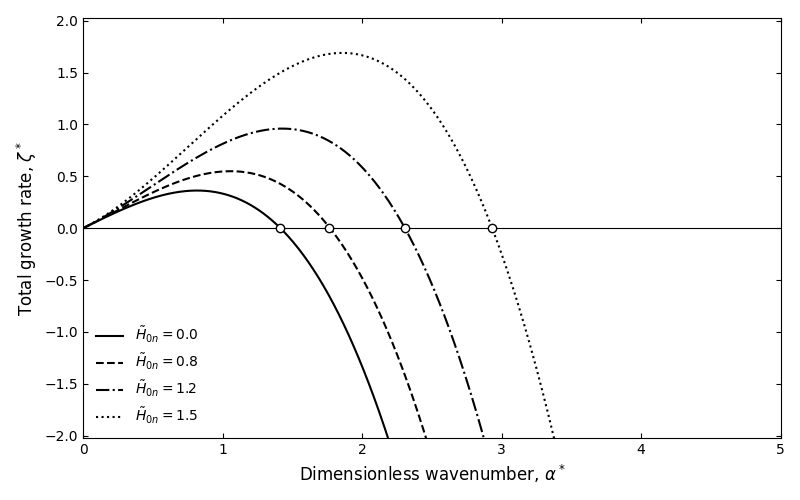
\includegraphics[width=0.5\linewidth]{figuras/lsa/Grafico-LSA-Impacto-de-H_n.png}
    \caption{Effect of a normal magnetic field $\tilde{H}_{0n}$ on the dimensionless dispersion relation. Increasing $\tilde{H}_{0n}$ amplifies the maximum growth rate and shifts the cut-off wavenumber to the right (destabilizing effect).}
    \label{fig:Grafico-LSA-Impacto-de-H_n}
\end{figure}

\begin{figure}
    \centering
    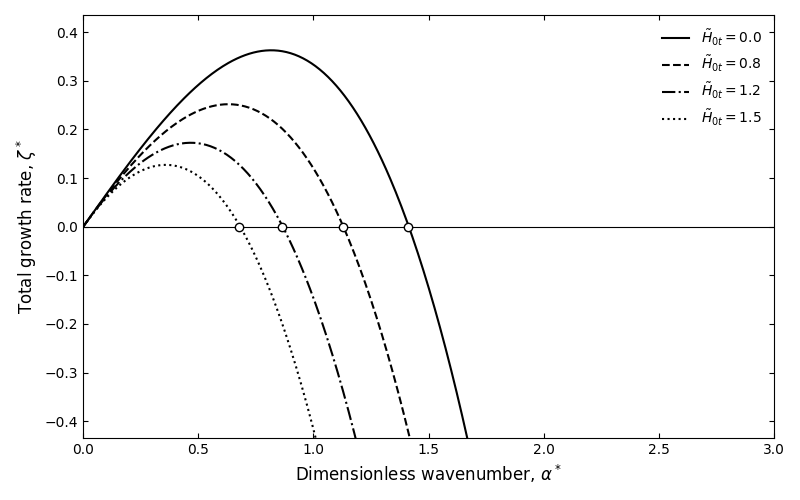
\includegraphics[width=0.5\linewidth]{figuras/lsa/Grafico-LSA-Impacto-de-H_t.png}
    \caption{Effect of a tangential magnetic field $\tilde{H}_{0t}$ on the dimensionless dispersion relation. Increasing $\tilde{H}_{0t}$ flattens the instability curve and shifts the cut-off wavenumber to the left (stabilizing effect).}
    \label{fig:Grafico-LSA-Impacto-de-H_t}
\end{figure}

Figures~\ref{fig:Grafico-LSA-Impacto-de-H_n} and~\ref{fig:Grafico-LSA-Impacto-de-H_t} compare the effects of applying a uniform magnetic field either normal ($\tilde{H}_{0n}$) or tangential ($\tilde{H}_{0t}$) to the fluid interface. The addition of the magnetic field introduces a quadratic term ($\propto {\alpha^*}^2$) to the dispersion relation, which alters the stability of the system depending entirely on the field's orientation.

When the magnetic field is normal to the interface (Figure~\ref{fig:Grafico-LSA-Impacto-de-H_n}), it acts as a strong destabilizing force. As $\tilde{H}_{0n}$ increases, the maximum growth rate is rapidly amplified, and the cut-off wavenumber shifts to the right. This indicates that the normal magnetic field overcomes the capillary forces, causing shorter wavelengths to become unstable and accelerating the overall deformation of the interface.

Conversely, when the magnetic field is tangential to the interface (Figure~\ref{fig:Grafico-LSA-Impacto-de-H_t}), it acts as a stabilizing mechanism. Increasing $\tilde{H}_{0t}$ decreases the growth rate, flattens the instability curve, and shifts the cut-off wavenumber to the left. In this configuration, the magnetic force works in the same direction as surface tension to suppress interfacial perturbations. This reduces the range of unstable waves and effectively delays the onset of the instability.

\begin{figure}
    \centering
    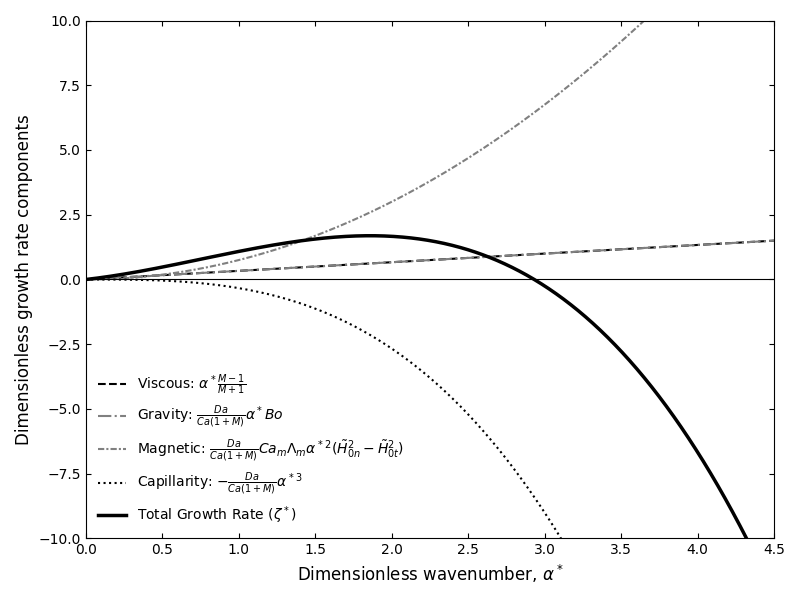
\includegraphics[width=0.5\linewidth]{figuras/lsa/Grafico-LSA-Impacto-de-todos-termos-MAG.png}
    \caption{Decomposition of the dimensionless dispersion relation under a dominant normal magnetic field ($\tilde{H}_{0n} > \tilde{H}_{0t}$) into its individual physical contributions: viscous forcing, gravity, magnetic (Kelvin) forcing, and capillarity.}
    \label{fig:Grafico-LSA-Impacto-de-todos-termos-MAG}
\end{figure}

Figure~\ref{fig:Grafico-LSA-Impacto-de-todos-termos-MAG} breaks down the individual physical forces that make up the total dispersion relation under a normal magnetic field ($\tilde{H}_{0n} > \tilde{H}_{0t}$). The total growth rate ($\zeta^*$) is the direct sum of four components: viscosity, gravity, the magnetic force, and capillarity. As the graph shows, the viscous and gravitational forces grow linearly with the dimensionless wavenumber ($\alpha^*$). However, the newly added magnetic force grows quadratically ($\propto {\alpha^*}^2$). Because of this steeper curve, the magnetic term quickly outpaces the linear forces, acting as a powerful amplifier that drives the interface into a highly unstable state at intermediate wavelengths. To counteract this rapid, accelerated growth, a stronger restoring force is required. Capillarity provides this balance because it scales with the negative cube of the wavenumber ($-{\alpha^*}^3$). Although it starts small, this cubic term eventually overpowers all three destabilizing forces at higher wavenumbers, forcing the total growth rate to drop sharply below zero and ensuring the interface remains stable against microscopic perturbations.